\documentclass[1p]{elsarticle_modified}
%\bibliographystyle{elsarticle-num}

%\usepackage[colorlinks]{hyperref}
%\usepackage{abbrmath_seonhwa} %\Abb, \Ascr, \Acal ,\Abf, \Afrak
\usepackage{amsfonts}
\usepackage{amssymb}
\usepackage{amsmath}
\usepackage{amsthm}
\usepackage{scalefnt}
\usepackage{amsbsy}
\usepackage{kotex}
\usepackage{caption}
\usepackage{subfig}
\usepackage{color}
\usepackage{graphicx}
\usepackage{xcolor} %% white, black, red, green, blue, cyan, magenta, yellow
\usepackage{float}
\usepackage{setspace}
\usepackage{hyperref}

\usepackage{tikz}
\usetikzlibrary{arrows}

\usepackage{multirow}
\usepackage{array} % fixed length table
\usepackage{hhline}

%%%%%%%%%%%%%%%%%%%%%
\makeatletter
\renewcommand*\env@matrix[1][\arraystretch]{%
	\edef\arraystretch{#1}%
	\hskip -\arraycolsep
	\let\@ifnextchar\new@ifnextchar
	\array{*\c@MaxMatrixCols c}}
\makeatother %https://tex.stackexchange.com/questions/14071/how-can-i-increase-the-line-spacing-in-a-matrix
%%%%%%%%%%%%%%%

\usepackage[normalem]{ulem}

\newcommand{\msout}[1]{\ifmmode\text{\sout{\ensuremath{#1}}}\else\sout{#1}\fi}
%SOURCE: \msout is \stkout macro in https://tex.stackexchange.com/questions/20609/strikeout-in-math-mode

\newcommand{\cancel}[1]{
	\ifmmode
	{\color{red}\msout{#1}}
	\else
	{\color{red}\sout{#1}}
	\fi
}

\newcommand{\add}[1]{
	{\color{blue}\uwave{#1}}
}

\newcommand{\replace}[2]{
	\ifmmode
	{\color{red}\msout{#1}}{\color{blue}\uwave{#2}}
	\else
	{\color{red}\sout{#1}}{\color{blue}\uwave{#2}}
	\fi
}

\newcommand{\Sol}{\mathcal{S}} %segment
\newcommand{\D}{D} %diagram
\newcommand{\A}{\mathcal{A}} %arc


%%%%%%%%%%%%%%%%%%%%%%%%%%%%%5 test

\def\sl{\operatorname{\textup{SL}}(2,\Cbb)}
\def\psl{\operatorname{\textup{PSL}}(2,\Cbb)}
\def\quan{\mkern 1mu \triangleright \mkern 1mu}

\theoremstyle{definition}
\newtheorem{thm}{Theorem}[section]
\newtheorem{prop}[thm]{Proposition}
\newtheorem{lem}[thm]{Lemma}
\newtheorem{ques}[thm]{Question}
\newtheorem{cor}[thm]{Corollary}
\newtheorem{defn}[thm]{Definition}
\newtheorem{exam}[thm]{Example}
\newtheorem{rmk}[thm]{Remark}
\newtheorem{alg}[thm]{Algorithm}

\newcommand{\I}{\sqrt{-1}}
\begin{document}

%\begin{frontmatter}
%
%\title{Boundary parabolic representations of knots up to 8 crossings}
%
%%% Group authors per affiliation:
%\author{Yunhi Cho} 
%\address{Department of Mathematics, University of Seoul, Seoul, Korea}
%\ead{yhcho@uos.ac.kr}
%
%
%\author{Seonhwa Kim} %\fnref{s_kim}}
%\address{Center for Geometry and Physics, Institute for Basic Science, Pohang, 37673, Korea}
%\ead{ryeona17@ibs.re.kr}
%
%\author{Hyuk Kim}
%\address{Department of Mathematical Sciences, Seoul National University, Seoul 08826, Korea}
%\ead{hyukkim@snu.ac.kr}
%
%\author{Seokbeom Yoon}
%\address{Department of Mathematical Sciences, Seoul National University, Seoul, 08826,  Korea}
%\ead{sbyoon15@snu.ac.kr}
%
%\begin{abstract}
%We find all boundary parabolic representation of knots up to 8 crossings.
%
%\end{abstract}
%\begin{keyword}
%    \MSC[2010] 57M25 
%\end{keyword}
%
%\end{frontmatter}

%\linenumbers
%\tableofcontents
%
\newcommand\colored[1]{\textcolor{white}{\rule[-0.35ex]{0.8em}{1.4ex}}\kern-0.8em\color{red} #1}%
%\newcommand\colored[1]{\textcolor{white}{ #1}\kern-2.17ex	\textcolor{white}{ #1}\kern-1.81ex	\textcolor{white}{ #1}\kern-2.15ex\color{red}#1	}

{\Large $\underline{12a_{0248}~(K12a_{0248})}$}

\setlength{\tabcolsep}{10pt}
\renewcommand{\arraystretch}{1.6}
\vspace{1cm}\begin{tabular}{m{100pt}>{\centering\arraybackslash}m{274pt}}
\multirow{5}{120pt}{
	\centering
	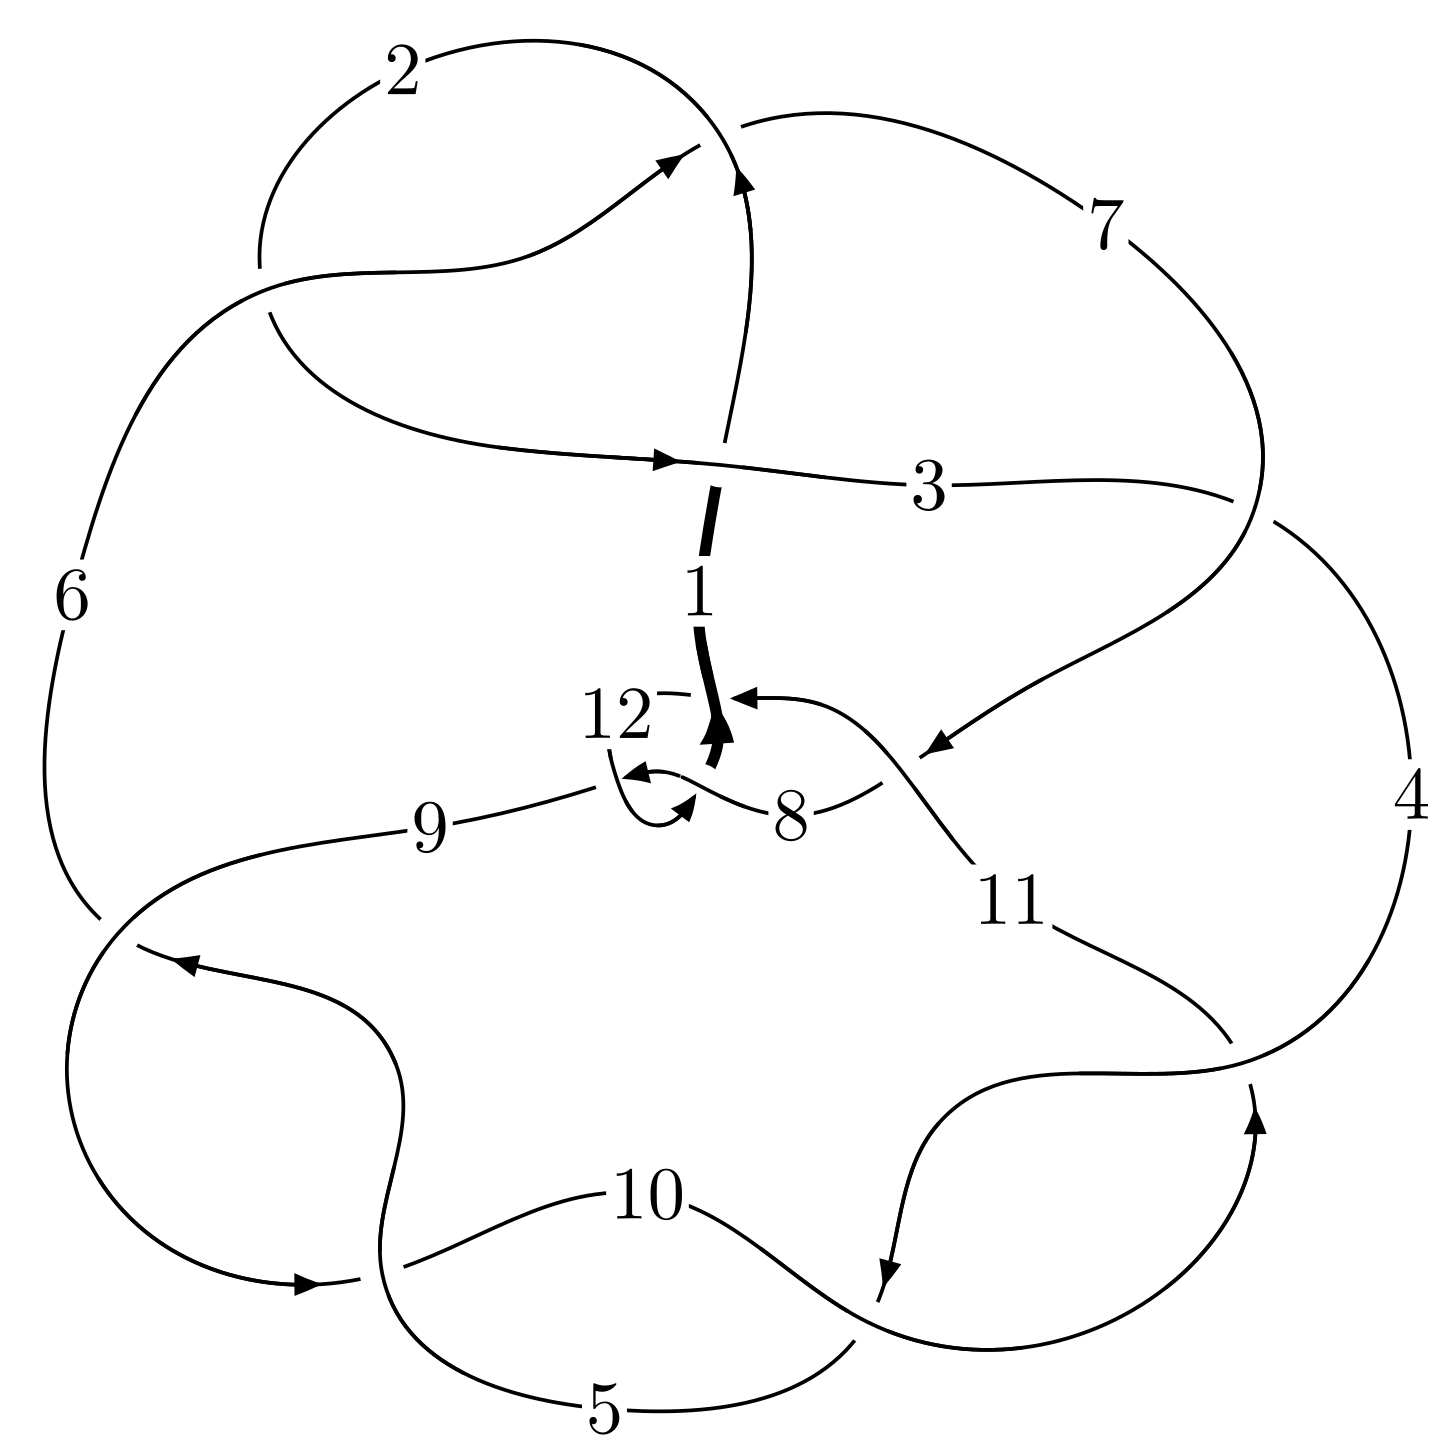
\includegraphics[width=112pt]{../../../GIT/diagram.site/Diagrams/png/1049_12a_0248.png}\\
\ \ \ A knot diagram\footnotemark}&
\allowdisplaybreaks
\textbf{Linearized knot diagam} \\
\cline{2-2}
 &
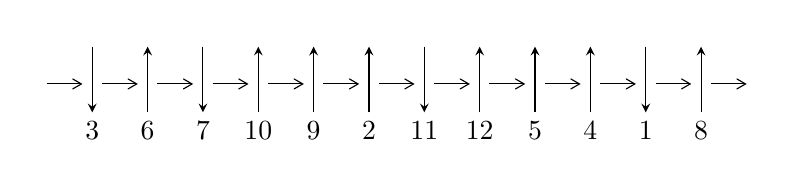
\begin{tikzpicture}[x=20pt, y=17pt]
	% nodes
	\node (C0) at (0, 0) {};
	\node (C1) at (1, 0) {};
	\node (C1U) at (1, +1) {};
	\node (C1D) at (1, -1) {3};

	\node (C2) at (2, 0) {};
	\node (C2U) at (2, +1) {};
	\node (C2D) at (2, -1) {6};

	\node (C3) at (3, 0) {};
	\node (C3U) at (3, +1) {};
	\node (C3D) at (3, -1) {7};

	\node (C4) at (4, 0) {};
	\node (C4U) at (4, +1) {};
	\node (C4D) at (4, -1) {10};

	\node (C5) at (5, 0) {};
	\node (C5U) at (5, +1) {};
	\node (C5D) at (5, -1) {9};

	\node (C6) at (6, 0) {};
	\node (C6U) at (6, +1) {};
	\node (C6D) at (6, -1) {2};

	\node (C7) at (7, 0) {};
	\node (C7U) at (7, +1) {};
	\node (C7D) at (7, -1) {11};

	\node (C8) at (8, 0) {};
	\node (C8U) at (8, +1) {};
	\node (C8D) at (8, -1) {12};

	\node (C9) at (9, 0) {};
	\node (C9U) at (9, +1) {};
	\node (C9D) at (9, -1) {5};

	\node (C10) at (10, 0) {};
	\node (C10U) at (10, +1) {};
	\node (C10D) at (10, -1) {4};

	\node (C11) at (11, 0) {};
	\node (C11U) at (11, +1) {};
	\node (C11D) at (11, -1) {1};

	\node (C12) at (12, 0) {};
	\node (C12U) at (12, +1) {};
	\node (C12D) at (12, -1) {8};
	\node (C13) at (13, 0) {};

	% arrows
	\draw[->,>={angle 60}]
	(C0) edge (C1) (C1) edge (C2) (C2) edge (C3) (C3) edge (C4) (C4) edge (C5) (C5) edge (C6) (C6) edge (C7) (C7) edge (C8) (C8) edge (C9) (C9) edge (C10) (C10) edge (C11) (C11) edge (C12) (C12) edge (C13) ;	\draw[->,>=stealth]
	(C1U) edge (C1D) (C2D) edge (C2U) (C3U) edge (C3D) (C4D) edge (C4U) (C5D) edge (C5U) (C6D) edge (C6U) (C7U) edge (C7D) (C8D) edge (C8U) (C9D) edge (C9U) (C10D) edge (C10U) (C11U) edge (C11D) (C12D) edge (C12U) ;
	\end{tikzpicture} \\
\hhline{~~} \\& 
\textbf{Solving Sequence} \\ \cline{2-2} 
 &
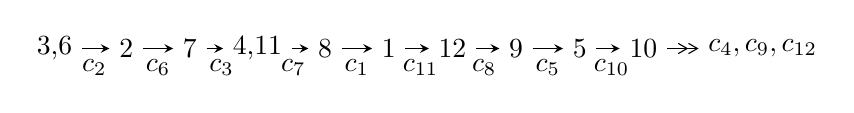
\begin{tikzpicture}[x=23pt, y=7pt]
	% node
	\node (A0) at (-1/8, 0) {3,6};
	\node (A1) at (1, 0) {2};
	\node (A2) at (2, 0) {7};
	\node (A3) at (49/16, 0) {4,11};
	\node (A4) at (33/8, 0) {8};
	\node (A5) at (41/8, 0) {1};
	\node (A6) at (49/8, 0) {12};
	\node (A7) at (57/8, 0) {9};
	\node (A8) at (65/8, 0) {5};
	\node (A9) at (73/8, 0) {10};
	\node (C1) at (1/2, -1) {$c_{2}$};
	\node (C2) at (3/2, -1) {$c_{6}$};
	\node (C3) at (5/2, -1) {$c_{3}$};
	\node (C4) at (29/8, -1) {$c_{7}$};
	\node (C5) at (37/8, -1) {$c_{1}$};
	\node (C6) at (45/8, -1) {$c_{11}$};
	\node (C7) at (53/8, -1) {$c_{8}$};
	\node (C8) at (61/8, -1) {$c_{5}$};
	\node (C9) at (69/8, -1) {$c_{10}$};
	\node (A10) at (11, 0) {$c_{4},c_{9},c_{12}$};

	% edge
	\draw[->,>=stealth]	
	(A0) edge (A1) (A1) edge (A2) (A2) edge (A3) (A3) edge (A4) (A4) edge (A5) (A5) edge (A6) (A6) edge (A7) (A7) edge (A8) (A8) edge (A9) ;
	\draw[->>,>={angle 60}]	
	(A9) edge (A10);
\end{tikzpicture} \\ 

\end{tabular} \\

\footnotetext{
The image of knot diagram is generated by the software ``\textbf{Draw programme}" developed by Andrew Bartholomew(\url{http://www.layer8.co.uk/maths/draw/index.htm\#Running-draw}), where we modified some parts for our purpose(\url{https://github.com/CATsTAILs/LinksPainter}).
}\phantom \\ \newline 
\centering \textbf{Ideals for irreducible components\footnotemark of $X_{\text{par}}$} 
 
\begin{align*}
I^u_{1}&=\langle 
u^{20}+u^{19}+\cdots-3 u^2+2 b,\;u^{20}+u^{19}+\cdots+2 a-1,\;u^{22}+u^{21}+\cdots+u+1\rangle \\
I^u_{2}&=\langle 
3.68754\times10^{30} u^{61}+8.39103\times10^{30} u^{60}+\cdots+2.19146\times10^{31} b-4.54412\times10^{30},\\
\phantom{I^u_{2}}&\phantom{= \langle  }5.62366\times10^{30} u^{61}+9.32012\times10^{29} u^{60}+\cdots+6.57438\times10^{31} a+1.25939\times10^{32},\;u^{62}+2 u^{61}+\cdots+7 u+3\rangle \\
I^u_{3}&=\langle 
- a u+b- u,\;a^2-2 u,\;u^2- u+1\rangle \\
I^u_{4}&=\langle 
b+u,\;a,\;u^2+u+1\rangle \\
I^u_{5}&=\langle 
- a u+b+1,\;a^2-2 u,\;u^2- u+1\rangle \\
I^u_{6}&=\langle 
b+1,\;a,\;u^2+u+1\rangle \\
\\
\end{align*}
\raggedright * 6 irreducible components of $\dim_{\mathbb{C}}=0$, with total 96 representations.\\
\footnotetext{All coefficients of polynomials are rational numbers. But the coefficients are sometimes approximated in decimal forms when there is not enough margin.}
\newpage
\renewcommand{\arraystretch}{1}
\centering \section*{I. $I^u_{1}= \langle u^{20}+u^{19}+\cdots-3 u^2+2 b,\;u^{20}+u^{19}+\cdots+2 a-1,\;u^{22}+u^{21}+\cdots+u+1 \rangle$}
\flushleft \textbf{(i) Arc colorings}\\
\begin{tabular}{m{7pt} m{180pt} m{7pt} m{180pt} }
\flushright $a_{3}=$&$\begin{pmatrix}1\\0\end{pmatrix}$ \\
\flushright $a_{6}=$&$\begin{pmatrix}0\\u\end{pmatrix}$ \\
\flushright $a_{2}=$&$\begin{pmatrix}1\\u^2\end{pmatrix}$ \\
\flushright $a_{7}=$&$\begin{pmatrix}u\\u^3+u\end{pmatrix}$ \\
\flushright $a_{4}=$&$\begin{pmatrix}u^4+u^2+1\\u^6+2 u^4+u^2\end{pmatrix}$ \\
\flushright $a_{11}=$&$\begin{pmatrix}-\frac{1}{2} u^{20}-\frac{1}{2} u^{19}+\cdots-\frac{1}{2} u+\frac{1}{2}\\-\frac{1}{2} u^{20}-\frac{1}{2} u^{19}+\cdots-\frac{1}{2} u^3+\frac{3}{2} u^2\end{pmatrix}$ \\
\flushright $a_{8}=$&$\begin{pmatrix}\frac{1}{2} u^{21}+\frac{1}{2} u^{20}+\cdots+\frac{1}{2} u^4-\frac{5}{2} u^3\\-\frac{1}{2} u^{19}-\frac{1}{2} u^{18}+\cdots-\frac{1}{2} u^2+\frac{1}{2} u\end{pmatrix}$ \\
\flushright $a_{1}=$&$\begin{pmatrix}u^2+1\\u^2\end{pmatrix}$ \\
\flushright $a_{12}=$&$\begin{pmatrix}-\frac{1}{2} u^{20}-\frac{1}{2} u^{19}+\cdots-\frac{1}{2} u+\frac{1}{2}\\-\frac{1}{2} u^{20}-\frac{1}{2} u^{19}+\cdots-\frac{1}{2} u^3+\frac{3}{2} u^2\end{pmatrix}$ \\
\flushright $a_{9}=$&$\begin{pmatrix}-\frac{1}{2} u^{19}-\frac{1}{2} u^{18}+\cdots-\frac{1}{2} u^2+\frac{1}{2} u\\-\frac{1}{2} u^{21}-\frac{1}{2} u^{20}+\cdots-\frac{1}{2} u^2+\frac{1}{2} u\end{pmatrix}$ \\
\flushright $a_{5}=$&$\begin{pmatrix}-\frac{1}{2} u^{20}- u^{19}+\cdots-2 u-\frac{1}{2}\\- u^{21}-\frac{3}{2} u^{20}+\cdots-2 u^2-\frac{1}{2} u\end{pmatrix}$ \\
\flushright $a_{10}=$&$\begin{pmatrix}-\frac{1}{2} u^{20}-\frac{1}{2} u^{19}+\cdots-\frac{1}{2} u+\frac{1}{2}\\-\frac{1}{2} u^{20}-\frac{1}{2} u^{19}+\cdots+\frac{1}{2} u+\frac{1}{2}\end{pmatrix}$\\&\end{tabular}
\flushleft \textbf{(ii) Obstruction class $= -1$}\\~\\
\flushleft \textbf{(iii) Cusp Shapes $= 5 u^{21}+u^{20}+29 u^{19}+u^{18}+79 u^{17}-5 u^{16}+115 u^{15}-19 u^{14}+79 u^{13}-18 u^{12}-5 u^{11}-30 u^9+8 u^8+15 u^7-18 u^6+37 u^5-17 u^4+11 u^3+1$}\\~\\
\newpage\renewcommand{\arraystretch}{1}
\flushleft \textbf{(iv) u-Polynomials at the component}\newline \\
\begin{tabular}{m{50pt}|m{274pt}}
Crossings & \hspace{64pt}u-Polynomials at each crossing \\
\hline $$\begin{aligned}c_{1},c_{11}\end{aligned}$$&$\begin{aligned}
&u^{22}+13 u^{21}+\cdots+3 u+1
\end{aligned}$\\
\hline $$\begin{aligned}c_{2},c_{6},c_{8}\\c_{12}\end{aligned}$$&$\begin{aligned}
&u^{22}- u^{21}+\cdots- u+1
\end{aligned}$\\
\hline $$\begin{aligned}c_{3},c_{7}\end{aligned}$$&$\begin{aligned}
&u^{22}+u^{21}+\cdots+u+1
\end{aligned}$\\
\hline $$\begin{aligned}c_{4},c_{5},c_{9}\\c_{10}\end{aligned}$$&$\begin{aligned}
&u^{22}-5 u^{21}+\cdots-24 u+4
\end{aligned}$\\
\hline
\end{tabular}\\~\\
\newpage\renewcommand{\arraystretch}{1}
\flushleft \textbf{(v) Riley Polynomials at the component}\newline \\
\begin{tabular}{m{50pt}|m{274pt}}
Crossings & \hspace{64pt}Riley Polynomials at each crossing \\
\hline $$\begin{aligned}c_{1},c_{11}\end{aligned}$$&$\begin{aligned}
&y^{22}-3 y^{21}+\cdots+11 y+1
\end{aligned}$\\
\hline $$\begin{aligned}c_{2},c_{6},c_{8}\\c_{12}\end{aligned}$$&$\begin{aligned}
&y^{22}+13 y^{21}+\cdots+3 y+1
\end{aligned}$\\
\hline $$\begin{aligned}c_{3},c_{7}\end{aligned}$$&$\begin{aligned}
&y^{22}-19 y^{21}+\cdots+3 y+1
\end{aligned}$\\
\hline $$\begin{aligned}c_{4},c_{5},c_{9}\\c_{10}\end{aligned}$$&$\begin{aligned}
&y^{22}+25 y^{21}+\cdots-32 y+16
\end{aligned}$\\
\hline
\end{tabular}\\~\\
\newpage\flushleft \textbf{(vi) Complex Volumes and Cusp Shapes}
$$\begin{array}{c|c|c}  
\text{Solutions to }I^u_{1}& \I (\text{vol} + \sqrt{-1}CS) & \text{Cusp shape}\\
 \hline 
\begin{aligned}
u &= \phantom{-}0.277173 + 1.020170 I \\
a &= -1.65615 - 0.40699 I \\
b &= \phantom{-}0.13433 - 1.51680 I\end{aligned}
 & -7.08694 + 3.87705 I & -7.21377 - 4.81561 I \\ \hline\begin{aligned}
u &= \phantom{-}0.277173 - 1.020170 I \\
a &= -1.65615 + 0.40699 I \\
b &= \phantom{-}0.13433 + 1.51680 I\end{aligned}
 & -7.08694 - 3.87705 I & -7.21377 + 4.81561 I \\ \hline\begin{aligned}
u &= -0.121456 + 0.889759 I \\
a &= -1.029430 - 0.242749 I \\
b &= -0.505192 + 0.384473 I\end{aligned}
 & -2.07127 - 1.48890 I & -2.67809 + 4.69847 I \\ \hline\begin{aligned}
u &= -0.121456 - 0.889759 I \\
a &= -1.029430 + 0.242749 I \\
b &= -0.505192 - 0.384473 I\end{aligned}
 & -2.07127 + 1.48890 I & -2.67809 - 4.69847 I \\ \hline\begin{aligned}
u &= -0.848934 + 0.255974 I \\
a &= \phantom{-}1.72949 - 0.07214 I \\
b &= \phantom{-}1.176080 - 0.436448 I\end{aligned}
 & -8.20167 + 4.95433 I & \phantom{-}1.91829 - 2.01188 I \\ \hline\begin{aligned}
u &= -0.848934 - 0.255974 I \\
a &= \phantom{-}1.72949 + 0.07214 I \\
b &= \phantom{-}1.176080 + 0.436448 I\end{aligned}
 & -8.20167 - 4.95433 I & \phantom{-}1.91829 + 2.01188 I \\ \hline\begin{aligned}
u &= \phantom{-}0.403077 + 1.151660 I \\
a &= -0.87654 - 1.38792 I \\
b &= \phantom{-}1.59601 - 1.51481 I\end{aligned}
 & -7.80702 + 4.05683 I & -5.44929 - 3.62162 I \\ \hline\begin{aligned}
u &= \phantom{-}0.403077 - 1.151660 I \\
a &= -0.87654 + 1.38792 I \\
b &= \phantom{-}1.59601 + 1.51481 I\end{aligned}
 & -7.80702 - 4.05683 I & -5.44929 + 3.62162 I \\ \hline\begin{aligned}
u &= \phantom{-}0.716845 + 0.261797 I \\
a &= \phantom{-}1.67749 + 0.17960 I \\
b &= \phantom{-}0.911783 + 0.513874 I\end{aligned}
 & -0.28086 - 2.78084 I & \phantom{-}4.54791 + 3.72037 I \\ \hline\begin{aligned}
u &= \phantom{-}0.716845 - 0.261797 I \\
a &= \phantom{-}1.67749 - 0.17960 I \\
b &= \phantom{-}0.911783 - 0.513874 I\end{aligned}
 & -0.28086 + 2.78084 I & \phantom{-}4.54791 - 3.72037 I\\
 \hline 
 \end{array}$$\newpage$$\begin{array}{c|c|c}  
\text{Solutions to }I^u_{1}& \I (\text{vol} + \sqrt{-1}CS) & \text{Cusp shape}\\
 \hline 
\begin{aligned}
u &= -0.498272 + 1.142550 I \\
a &= -0.43520 + 1.93340 I \\
b &= \phantom{-}2.28341 + 1.52363 I\end{aligned}
 & -3.73649 - 7.94900 I & -0.13573 + 6.16396 I \\ \hline\begin{aligned}
u &= -0.498272 - 1.142550 I \\
a &= -0.43520 - 1.93340 I \\
b &= \phantom{-}2.28341 - 1.52363 I\end{aligned}
 & -3.73649 + 7.94900 I & -0.13573 - 6.16396 I \\ \hline\begin{aligned}
u &= \phantom{-}0.444842 + 0.593309 I \\
a &= \phantom{-}1.42127 + 1.52607 I \\
b &= -0.44921 + 1.51322 I\end{aligned}
 & -4.25955 + 2.40332 I & \phantom{-}2.42276 - 1.87700 I \\ \hline\begin{aligned}
u &= \phantom{-}0.444842 - 0.593309 I \\
a &= \phantom{-}1.42127 - 1.52607 I \\
b &= -0.44921 - 1.51322 I\end{aligned}
 & -4.25955 - 2.40332 I & \phantom{-}2.42276 + 1.87700 I \\ \hline\begin{aligned}
u &= \phantom{-}0.551692 + 1.163780 I \\
a &= -0.01034 - 1.91326 I \\
b &= \phantom{-}2.50735 - 1.20167 I\end{aligned}
 & -5.50564 + 12.55900 I & -1.64021 - 10.10675 I \\ \hline\begin{aligned}
u &= \phantom{-}0.551692 - 1.163780 I \\
a &= -0.01034 + 1.91326 I \\
b &= \phantom{-}2.50735 + 1.20167 I\end{aligned}
 & -5.50564 - 12.55900 I & -1.64021 + 10.10675 I \\ \hline\begin{aligned}
u &= -0.335392 + 1.264210 I \\
a &= -0.530073 + 0.859819 I \\
b &= \phantom{-}1.47236 + 0.87987 I\end{aligned}
 & -17.5375 - 2.7555 I & -7.01676 + 2.91273 I \\ \hline\begin{aligned}
u &= -0.335392 - 1.264210 I \\
a &= -0.530073 - 0.859819 I \\
b &= \phantom{-}1.47236 - 0.87987 I\end{aligned}
 & -17.5375 + 2.7555 I & -7.01676 - 2.91273 I \\ \hline\begin{aligned}
u &= -0.591533 + 1.189200 I \\
a &= \phantom{-}0.24537 + 1.77352 I \\
b &= \phantom{-}2.54369 + 0.94767 I\end{aligned}
 & -13.6900 - 15.6170 I & -3.36409 + 8.79372 I \\ \hline\begin{aligned}
u &= -0.591533 - 1.189200 I \\
a &= \phantom{-}0.24537 - 1.77352 I \\
b &= \phantom{-}2.54369 - 0.94767 I\end{aligned}
 & -13.6900 + 15.6170 I & -3.36409 - 8.79372 I\\
 \hline 
 \end{array}$$\newpage$$\begin{array}{c|c|c}  
\text{Solutions to }I^u_{1}& \I (\text{vol} + \sqrt{-1}CS) & \text{Cusp shape}\\
 \hline 
\begin{aligned}
u &= -0.498042 + 0.364034 I \\
a &= \phantom{-}1.46412 - 0.51940 I \\
b &= \phantom{-}0.329394 - 0.747695 I\end{aligned}
 & \phantom{-}1.089740 - 0.536721 I & \phantom{-}8.60899 + 3.28109 I \\ \hline\begin{aligned}
u &= -0.498042 - 0.364034 I \\
a &= \phantom{-}1.46412 + 0.51940 I \\
b &= \phantom{-}0.329394 + 0.747695 I\end{aligned}
 & \phantom{-}1.089740 + 0.536721 I & \phantom{-}8.60899 - 3.28109 I\\
 \hline 
 \end{array}$$\newpage\newpage\renewcommand{\arraystretch}{1}
\centering \section*{II. $I^u_{2}= \langle 3.69\times10^{30} u^{61}+8.39\times10^{30} u^{60}+\cdots+2.19\times10^{31} b-4.54\times10^{30},\;5.62\times10^{30} u^{61}+9.32\times10^{29} u^{60}+\cdots+6.57\times10^{31} a+1.26\times10^{32},\;u^{62}+2 u^{61}+\cdots+7 u+3 \rangle$}
\flushleft \textbf{(i) Arc colorings}\\
\begin{tabular}{m{7pt} m{180pt} m{7pt} m{180pt} }
\flushright $a_{3}=$&$\begin{pmatrix}1\\0\end{pmatrix}$ \\
\flushright $a_{6}=$&$\begin{pmatrix}0\\u\end{pmatrix}$ \\
\flushright $a_{2}=$&$\begin{pmatrix}1\\u^2\end{pmatrix}$ \\
\flushright $a_{7}=$&$\begin{pmatrix}u\\u^3+u\end{pmatrix}$ \\
\flushright $a_{4}=$&$\begin{pmatrix}u^4+u^2+1\\u^6+2 u^4+u^2\end{pmatrix}$ \\
\flushright $a_{11}=$&$\begin{pmatrix}-0.0855391 u^{61}-0.0141764 u^{60}+\cdots-4.70351 u-1.91561\\-0.168269 u^{61}-0.382897 u^{60}+\cdots-2.55324 u+0.207356\end{pmatrix}$ \\
\flushright $a_{8}=$&$\begin{pmatrix}-0.784652 u^{61}-1.03466 u^{60}+\cdots-6.06002 u-3.97213\\-0.416695 u^{61}+0.167342 u^{60}+\cdots+4.79125 u+3.54242\end{pmatrix}$ \\
\flushright $a_{1}=$&$\begin{pmatrix}u^2+1\\u^2\end{pmatrix}$ \\
\flushright $a_{12}=$&$\begin{pmatrix}-0.0402708 u^{61}+0.447531 u^{60}+\cdots-3.91890 u-2.58902\\-0.267323 u^{61}-0.161926 u^{60}+\cdots-2.65084 u+0.351084\end{pmatrix}$ \\
\flushright $a_{9}=$&$\begin{pmatrix}-0.291785 u^{61}-0.157841 u^{60}+\cdots-2.92917 u-3.12929\\0.0849651 u^{61}+0.650458 u^{60}+\cdots+0.142039 u+0.688054\end{pmatrix}$ \\
\flushright $a_{5}=$&$\begin{pmatrix}-0.890090 u^{61}-2.38676 u^{60}+\cdots-9.65587 u-6.58484\\0.381623 u^{61}-0.451639 u^{60}+\cdots+1.38007 u+0.627994\end{pmatrix}$ \\
\flushright $a_{10}=$&$\begin{pmatrix}-0.223944 u^{61}+0.335268 u^{60}+\cdots-2.74033 u-3.36849\\-0.480269 u^{61}-0.308145 u^{60}+\cdots-1.68366 u-0.00366767\end{pmatrix}$\\&\end{tabular}
\flushleft \textbf{(ii) Obstruction class $= -1$}\\~\\
\flushleft \textbf{(iii) Cusp Shapes $= 2.13514 u^{61}+3.90356 u^{60}+\cdots+2.88438 u-1.52833$}\\~\\
\newpage\renewcommand{\arraystretch}{1}
\flushleft \textbf{(iv) u-Polynomials at the component}\newline \\
\begin{tabular}{m{50pt}|m{274pt}}
Crossings & \hspace{64pt}u-Polynomials at each crossing \\
\hline $$\begin{aligned}c_{1},c_{11}\end{aligned}$$&$\begin{aligned}
&u^{62}+30 u^{61}+\cdots+35 u+9
\end{aligned}$\\
\hline $$\begin{aligned}c_{2},c_{6},c_{8}\\c_{12}\end{aligned}$$&$\begin{aligned}
&u^{62}-2 u^{61}+\cdots-7 u+3
\end{aligned}$\\
\hline $$\begin{aligned}c_{3},c_{7}\end{aligned}$$&$\begin{aligned}
&u^{62}+2 u^{61}+\cdots-10747 u+14583
\end{aligned}$\\
\hline $$\begin{aligned}c_{4},c_{5},c_{9}\\c_{10}\end{aligned}$$&$\begin{aligned}
&(u^{31}+2 u^{30}+\cdots-8 u-2)^{2}
\end{aligned}$\\
\hline
\end{tabular}\\~\\
\newpage\renewcommand{\arraystretch}{1}
\flushleft \textbf{(v) Riley Polynomials at the component}\newline \\
\begin{tabular}{m{50pt}|m{274pt}}
Crossings & \hspace{64pt}Riley Polynomials at each crossing \\
\hline $$\begin{aligned}c_{1},c_{11}\end{aligned}$$&$\begin{aligned}
&y^{62}+6 y^{61}+\cdots-1009 y+81
\end{aligned}$\\
\hline $$\begin{aligned}c_{2},c_{6},c_{8}\\c_{12}\end{aligned}$$&$\begin{aligned}
&y^{62}+30 y^{61}+\cdots+35 y+9
\end{aligned}$\\
\hline $$\begin{aligned}c_{3},c_{7}\end{aligned}$$&$\begin{aligned}
&y^{62}-18 y^{61}+\cdots+711358091 y+212663889
\end{aligned}$\\
\hline $$\begin{aligned}c_{4},c_{5},c_{9}\\c_{10}\end{aligned}$$&$\begin{aligned}
&(y^{31}+38 y^{30}+\cdots-48 y-4)^{2}
\end{aligned}$\\
\hline
\end{tabular}\\~\\
\newpage\flushleft \textbf{(vi) Complex Volumes and Cusp Shapes}
$$\begin{array}{c|c|c}  
\text{Solutions to }I^u_{2}& \I (\text{vol} + \sqrt{-1}CS) & \text{Cusp shape}\\
 \hline 
\begin{aligned}
u &= -0.666104 + 0.730543 I \\
a &= \phantom{-}0.087322 + 0.584354 I \\
b &= \phantom{-}0.496094 - 0.738057 I\end{aligned}
 & -0.36232 - 5.51796 I & \phantom{-}0.77837 + 9.61169 I \\ \hline\begin{aligned}
u &= -0.666104 - 0.730543 I \\
a &= \phantom{-}0.087322 - 0.584354 I \\
b &= \phantom{-}0.496094 + 0.738057 I\end{aligned}
 & -0.36232 + 5.51796 I & \phantom{-}0.77837 - 9.61169 I \\ \hline\begin{aligned}
u &= \phantom{-}0.686447 + 0.784394 I \\
a &= \phantom{-}0.440237 + 0.732627 I \\
b &= -0.108205 + 0.403174 I\end{aligned}
 & -5.20347 + 2.59275 I & \phantom{-}2.06256 - 3.16265 I \\ \hline\begin{aligned}
u &= \phantom{-}0.686447 - 0.784394 I \\
a &= \phantom{-}0.440237 - 0.732627 I \\
b &= -0.108205 - 0.403174 I\end{aligned}
 & -5.20347 - 2.59275 I & \phantom{-}2.06256 + 3.16265 I \\ \hline\begin{aligned}
u &= -0.896489 + 0.288317 I \\
a &= -2.09267 - 0.04312 I \\
b &= -1.76964 + 0.85544 I\end{aligned}
 & -10.9647 + 10.1676 I & -0.91392 - 5.40901 I \\ \hline\begin{aligned}
u &= -0.896489 - 0.288317 I \\
a &= -2.09267 + 0.04312 I \\
b &= -1.76964 - 0.85544 I\end{aligned}
 & -10.9647 - 10.1676 I & -0.91392 + 5.40901 I \\ \hline\begin{aligned}
u &= -0.629178 + 0.873889 I \\
a &= -0.199672 - 0.056127 I \\
b &= -1.082620 - 0.085481 I\end{aligned}
 & -0.779034 + 0.507247 I & \phantom{-0.000000 } 0. - 2.93446 I \\ \hline\begin{aligned}
u &= -0.629178 - 0.873889 I \\
a &= -0.199672 + 0.056127 I \\
b &= -1.082620 + 0.085481 I\end{aligned}
 & -0.779034 - 0.507247 I & \phantom{-0.000000 -}0. + 2.93446 I \\ \hline\begin{aligned}
u &= \phantom{-}0.449825 + 0.996232 I \\
a &= -0.050283 - 0.198043 I \\
b &= -1.082620 - 0.085481 I\end{aligned}
 & -0.779034 + 0.507247 I & \phantom{-0.000000 } 0 \\ \hline\begin{aligned}
u &= \phantom{-}0.449825 - 0.996232 I \\
a &= -0.050283 + 0.198043 I \\
b &= -1.082620 + 0.085481 I\end{aligned}
 & -0.779034 - 0.507247 I & \phantom{-0.000000 } 0\\
 \hline 
 \end{array}$$\newpage$$\begin{array}{c|c|c}  
\text{Solutions to }I^u_{2}& \I (\text{vol} + \sqrt{-1}CS) & \text{Cusp shape}\\
 \hline 
\begin{aligned}
u &= -0.890494 + 0.168471 I \\
a &= -1.321460 - 0.466064 I \\
b &= -1.36135 - 0.59633 I\end{aligned}
 & -12.95390 + 1.38125 I & -3.10767 + 0.27219 I \\ \hline\begin{aligned}
u &= -0.890494 - 0.168471 I \\
a &= -1.321460 + 0.466064 I \\
b &= -1.36135 + 0.59633 I\end{aligned}
 & -12.95390 - 1.38125 I & -3.10767 - 0.27219 I \\ \hline\begin{aligned}
u &= \phantom{-}0.788781 + 0.767503 I \\
a &= \phantom{-}0.238484 - 0.701341 I \\
b &= \phantom{-}0.558659 + 0.646395 I\end{aligned}
 & -7.97068 + 6.77480 I & \phantom{-0.000000 } 0. - 6.34396 I \\ \hline\begin{aligned}
u &= \phantom{-}0.788781 - 0.767503 I \\
a &= \phantom{-}0.238484 + 0.701341 I \\
b &= \phantom{-}0.558659 - 0.646395 I\end{aligned}
 & -7.97068 - 6.77480 I & \phantom{-0.000000 -}0. + 6.34396 I \\ \hline\begin{aligned}
u &= -0.563357 + 0.949810 I \\
a &= \phantom{-}0.400448 - 0.334162 I \\
b &= \phantom{-}0.360204 - 0.897228 I\end{aligned}
 & \phantom{-}0.38775 - 3.17615 I & \phantom{-0.000000 } 0 \\ \hline\begin{aligned}
u &= -0.563357 - 0.949810 I \\
a &= \phantom{-}0.400448 + 0.334162 I \\
b &= \phantom{-}0.360204 + 0.897228 I\end{aligned}
 & \phantom{-}0.38775 + 3.17615 I & \phantom{-0.000000 } 0 \\ \hline\begin{aligned}
u &= \phantom{-}0.550433 + 0.959763 I \\
a &= \phantom{-}1.297360 + 0.482083 I \\
b &= \phantom{-}0.29971 + 1.71948 I\end{aligned}
 & -5.29982 + 1.79874 I & \phantom{-0.000000 } 0 \\ \hline\begin{aligned}
u &= \phantom{-}0.550433 - 0.959763 I \\
a &= \phantom{-}1.297360 - 0.482083 I \\
b &= \phantom{-}0.29971 - 1.71948 I\end{aligned}
 & -5.29982 - 1.79874 I & \phantom{-0.000000 } 0 \\ \hline\begin{aligned}
u &= -0.586824 + 0.636146 I \\
a &= \phantom{-}0.495132 - 0.651002 I \\
b &= -0.374983 - 0.161852 I\end{aligned}
 & \phantom{-}1.31051 - 1.39768 I & \phantom{-}6.56379 + 5.41262 I \\ \hline\begin{aligned}
u &= -0.586824 - 0.636146 I \\
a &= \phantom{-}0.495132 + 0.651002 I \\
b &= -0.374983 + 0.161852 I\end{aligned}
 & \phantom{-}1.31051 + 1.39768 I & \phantom{-}6.56379 - 5.41262 I\\
 \hline 
 \end{array}$$\newpage$$\begin{array}{c|c|c}  
\text{Solutions to }I^u_{2}& \I (\text{vol} + \sqrt{-1}CS) & \text{Cusp shape}\\
 \hline 
\begin{aligned}
u &= \phantom{-}0.491654 + 1.034130 I \\
a &= \phantom{-}0.074800 + 0.504612 I \\
b &= \phantom{-}0.496094 + 0.738057 I\end{aligned}
 & -0.36232 + 5.51796 I & \phantom{-0.000000 } 0 \\ \hline\begin{aligned}
u &= \phantom{-}0.491654 - 1.034130 I \\
a &= \phantom{-}0.074800 - 0.504612 I \\
b &= \phantom{-}0.496094 - 0.738057 I\end{aligned}
 & -0.36232 - 5.51796 I & \phantom{-0.000000 } 0 \\ \hline\begin{aligned}
u &= \phantom{-}0.801270 + 0.256679 I \\
a &= -2.23504 - 0.16817 I \\
b &= -1.66877 - 0.97408 I\end{aligned}
 & -2.82013 - 7.52476 I & \phantom{-}1.18698 + 6.99451 I \\ \hline\begin{aligned}
u &= \phantom{-}0.801270 - 0.256679 I \\
a &= -2.23504 + 0.16817 I \\
b &= -1.66877 + 0.97408 I\end{aligned}
 & -2.82013 + 7.52476 I & \phantom{-}1.18698 - 6.99451 I \\ \hline\begin{aligned}
u &= \phantom{-}0.323535 + 1.114360 I \\
a &= \phantom{-}0.075800 + 1.078080 I \\
b &= -1.27158 + 0.73117 I\end{aligned}
 & -4.23586 + 0.27259 I & \phantom{-0.000000 } 0 \\ \hline\begin{aligned}
u &= \phantom{-}0.323535 - 1.114360 I \\
a &= \phantom{-}0.075800 - 1.078080 I \\
b &= -1.27158 - 0.73117 I\end{aligned}
 & -4.23586 - 0.27259 I & \phantom{-0.000000 } 0 \\ \hline\begin{aligned}
u &= \phantom{-}0.750659 + 0.887428 I \\
a &= -0.358620 + 0.042820 I \\
b &= -1.162170 + 0.126258 I\end{aligned}
 & -8.32783 - 1.04707 I & \phantom{-0.000000 } 0 \\ \hline\begin{aligned}
u &= \phantom{-}0.750659 - 0.887428 I \\
a &= -0.358620 - 0.042820 I \\
b &= -1.162170 - 0.126258 I\end{aligned}
 & -8.32783 + 1.04707 I & \phantom{-0.000000 } 0 \\ \hline\begin{aligned}
u &= -0.472572 + 1.082310 I \\
a &= \phantom{-}0.148446 - 1.393170 I \\
b &= -1.41819 - 1.05546 I\end{aligned}
 & -0.99698 - 3.48995 I & \phantom{-0.000000 } 0 \\ \hline\begin{aligned}
u &= -0.472572 - 1.082310 I \\
a &= \phantom{-}0.148446 + 1.393170 I \\
b &= -1.41819 + 1.05546 I\end{aligned}
 & -0.99698 + 3.48995 I & \phantom{-0.000000 } 0\\
 \hline 
 \end{array}$$\newpage$$\begin{array}{c|c|c}  
\text{Solutions to }I^u_{2}& \I (\text{vol} + \sqrt{-1}CS) & \text{Cusp shape}\\
 \hline 
\begin{aligned}
u &= -0.387583 + 1.137140 I \\
a &= \phantom{-}0.60373 + 1.77130 I \\
b &= \phantom{-}1.90030\phantom{ +0.000000I}\end{aligned}
 & -4.52090\phantom{ +0.000000I} & \phantom{-0.000000 } 0 \\ \hline\begin{aligned}
u &= -0.387583 - 1.137140 I \\
a &= \phantom{-}0.60373 - 1.77130 I \\
b &= \phantom{-}1.90030\phantom{ +0.000000I}\end{aligned}
 & -4.52090\phantom{ +0.000000I} & \phantom{-0.000000 } 0 \\ \hline\begin{aligned}
u &= -0.426409 + 1.129220 I \\
a &= -0.131838 + 0.321832 I \\
b &= -1.162170 + 0.126258 I\end{aligned}
 & -8.32783 - 1.04707 I & \phantom{-0.000000 } 0 \\ \hline\begin{aligned}
u &= -0.426409 - 1.129220 I \\
a &= -0.131838 - 0.321832 I \\
b &= -1.162170 - 0.126258 I\end{aligned}
 & -8.32783 + 1.04707 I & \phantom{-0.000000 } 0 \\ \hline\begin{aligned}
u &= \phantom{-}0.291515 + 1.180250 I \\
a &= \phantom{-}0.23307 - 1.67452 I \\
b &= \phantom{-}1.65227 - 0.33136 I\end{aligned}
 & -7.28291 - 4.17154 I & \phantom{-0.000000 } 0 \\ \hline\begin{aligned}
u &= \phantom{-}0.291515 - 1.180250 I \\
a &= \phantom{-}0.23307 + 1.67452 I \\
b &= \phantom{-}1.65227 + 0.33136 I\end{aligned}
 & -7.28291 + 4.17154 I & \phantom{-0.000000 } 0 \\ \hline\begin{aligned}
u &= -0.475171 + 1.135050 I \\
a &= \phantom{-}0.049532 - 0.660701 I \\
b &= \phantom{-}0.558659 - 0.646395 I\end{aligned}
 & -7.97068 - 6.77480 I & \phantom{-0.000000 } 0 \\ \hline\begin{aligned}
u &= -0.475171 - 1.135050 I \\
a &= \phantom{-}0.049532 + 0.660701 I \\
b &= \phantom{-}0.558659 + 0.646395 I\end{aligned}
 & -7.97068 + 6.77480 I & \phantom{-0.000000 } 0 \\ \hline\begin{aligned}
u &= \phantom{-}0.418242 + 0.627505 I \\
a &= -0.559898 - 0.519466 I \\
b &= \phantom{-}0.360204 + 0.897228 I\end{aligned}
 & \phantom{-}0.38775 + 3.17615 I & \phantom{-}4.19909 + 0.89025 I \\ \hline\begin{aligned}
u &= \phantom{-}0.418242 - 0.627505 I \\
a &= -0.559898 + 0.519466 I \\
b &= \phantom{-}0.360204 - 0.897228 I\end{aligned}
 & \phantom{-}0.38775 - 3.17615 I & \phantom{-}4.19909 - 0.89025 I\\
 \hline 
 \end{array}$$\newpage$$\begin{array}{c|c|c}  
\text{Solutions to }I^u_{2}& \I (\text{vol} + \sqrt{-1}CS) & \text{Cusp shape}\\
 \hline 
\begin{aligned}
u &= \phantom{-}0.530235 + 1.136730 I \\
a &= -0.07716 + 1.50150 I \\
b &= -1.66877 + 0.97408 I\end{aligned}
 & -2.82013 + 7.52476 I & \phantom{-0.000000 } 0 \\ \hline\begin{aligned}
u &= \phantom{-}0.530235 - 1.136730 I \\
a &= -0.07716 - 1.50150 I \\
b &= -1.66877 - 0.97408 I\end{aligned}
 & -2.82013 - 7.52476 I & \phantom{-0.000000 } 0 \\ \hline\begin{aligned}
u &= \phantom{-}0.477297 + 1.164540 I \\
a &= \phantom{-}0.77266 - 1.43879 I \\
b &= \phantom{-}1.65227 + 0.33136 I\end{aligned}
 & -7.28291 + 4.17154 I & \phantom{-0.000000 } 0 \\ \hline\begin{aligned}
u &= \phantom{-}0.477297 - 1.164540 I \\
a &= \phantom{-}0.77266 + 1.43879 I \\
b &= \phantom{-}1.65227 - 0.33136 I\end{aligned}
 & -7.28291 - 4.17154 I & \phantom{-0.000000 } 0 \\ \hline\begin{aligned}
u &= -0.278446 + 1.228190 I \\
a &= -0.071389 - 1.005860 I \\
b &= -1.36135 - 0.59633 I\end{aligned}
 & -12.95390 + 1.38125 I & \phantom{-0.000000 } 0 \\ \hline\begin{aligned}
u &= -0.278446 - 1.228190 I \\
a &= -0.071389 + 1.005860 I \\
b &= -1.36135 + 0.59633 I\end{aligned}
 & -12.95390 - 1.38125 I & \phantom{-0.000000 } 0 \\ \hline\begin{aligned}
u &= \phantom{-}0.722560 + 0.106633 I \\
a &= -1.50741 + 0.82209 I \\
b &= -1.27158 + 0.73117 I\end{aligned}
 & -4.23586 + 0.27259 I & -1.68227 + 0.33399 I \\ \hline\begin{aligned}
u &= \phantom{-}0.722560 - 0.106633 I \\
a &= -1.50741 - 0.82209 I \\
b &= -1.27158 - 0.73117 I\end{aligned}
 & -4.23586 - 0.27259 I & -1.68227 - 0.33399 I \\ \hline\begin{aligned}
u &= -0.240118 + 1.264390 I \\
a &= \phantom{-}0.15678 + 1.45730 I \\
b &= \phantom{-}1.40042 + 0.34149 I\end{aligned}
 & -16.1317 + 6.5577 I & \phantom{-0.000000 } 0 \\ \hline\begin{aligned}
u &= -0.240118 - 1.264390 I \\
a &= \phantom{-}0.15678 - 1.45730 I \\
b &= \phantom{-}1.40042 - 0.34149 I\end{aligned}
 & -16.1317 - 6.5577 I & \phantom{-0.000000 } 0\\
 \hline 
 \end{array}$$\newpage$$\begin{array}{c|c|c}  
\text{Solutions to }I^u_{2}& \I (\text{vol} + \sqrt{-1}CS) & \text{Cusp shape}\\
 \hline 
\begin{aligned}
u &= -0.566003 + 1.180140 I \\
a &= -0.23494 - 1.48755 I \\
b &= -1.76964 - 0.85544 I\end{aligned}
 & -10.9647 - 10.1676 I & \phantom{-0.000000 } 0 \\ \hline\begin{aligned}
u &= -0.566003 - 1.180140 I \\
a &= -0.23494 + 1.48755 I \\
b &= -1.76964 + 0.85544 I\end{aligned}
 & -10.9647 + 10.1676 I & \phantom{-0.000000 } 0 \\ \hline\begin{aligned}
u &= -0.664612 + 0.170734 I \\
a &= -2.32627 + 0.63475 I \\
b &= -1.41819 + 1.05546 I\end{aligned}
 & -0.99698 + 3.48995 I & \phantom{-}4.01270 - 2.89115 I \\ \hline\begin{aligned}
u &= -0.664612 - 0.170734 I \\
a &= -2.32627 - 0.63475 I \\
b &= -1.41819 - 1.05546 I\end{aligned}
 & -0.99698 - 3.48995 I & \phantom{-}4.01270 + 2.89115 I \\ \hline\begin{aligned}
u &= \phantom{-}0.501484 + 0.456925 I \\
a &= \phantom{-}0.826582 + 0.636737 I \\
b &= -0.374983 - 0.161852 I\end{aligned}
 & \phantom{-}1.31051 - 1.39768 I & \phantom{-}6.56379 + 5.41262 I \\ \hline\begin{aligned}
u &= \phantom{-}0.501484 - 0.456925 I \\
a &= \phantom{-}0.826582 - 0.636737 I \\
b &= -0.374983 + 0.161852 I\end{aligned}
 & \phantom{-}1.31051 + 1.39768 I & \phantom{-}6.56379 - 5.41262 I \\ \hline\begin{aligned}
u &= -0.536448 + 1.217100 I \\
a &= \phantom{-}0.67450 + 1.24755 I \\
b &= \phantom{-}1.40042 - 0.34149 I\end{aligned}
 & -16.1317 - 6.5577 I & \phantom{-0.000000 } 0 \\ \hline\begin{aligned}
u &= -0.536448 - 1.217100 I \\
a &= \phantom{-}0.67450 - 1.24755 I \\
b &= \phantom{-}1.40042 + 0.34149 I\end{aligned}
 & -16.1317 + 6.5577 I & \phantom{-0.000000 } 0 \\ \hline\begin{aligned}
u &= \phantom{-}0.078963 + 0.630242 I \\
a &= -2.31047 - 0.68841 I \\
b &= \phantom{-}0.29971 - 1.71948 I\end{aligned}
 & -5.29982 - 1.79874 I & -2.21614 + 3.31862 I \\ \hline\begin{aligned}
u &= \phantom{-}0.078963 - 0.630242 I \\
a &= -2.31047 + 0.68841 I \\
b &= \phantom{-}0.29971 + 1.71948 I\end{aligned}
 & -5.29982 + 1.79874 I & -2.21614 - 3.31862 I\\
 \hline 
 \end{array}$$\newpage$$\begin{array}{c|c|c}  
\text{Solutions to }I^u_{2}& \I (\text{vol} + \sqrt{-1}CS) & \text{Cusp shape}\\
 \hline 
\begin{aligned}
u &= -0.583093 + 0.120029 I \\
a &= \phantom{-}0.73556 - 1.30329 I \\
b &= -0.108205 + 0.403174 I\end{aligned}
 & -5.20347 + 2.59275 I & \phantom{-}2.06256 - 3.16265 I \\ \hline\begin{aligned}
u &= -0.583093 - 0.120029 I \\
a &= \phantom{-}0.73556 + 1.30329 I \\
b &= -0.108205 - 0.403174 I\end{aligned}
 & -5.20347 - 2.59275 I & \phantom{-}2.06256 + 3.16265 I\\
 \hline 
 \end{array}$$\newpage\newpage\renewcommand{\arraystretch}{1}
\centering \section*{III. $I^u_{3}= \langle - a u+b- u,\;a^2-2 u,\;u^2- u+1 \rangle$}
\flushleft \textbf{(i) Arc colorings}\\
\begin{tabular}{m{7pt} m{180pt} m{7pt} m{180pt} }
\flushright $a_{3}=$&$\begin{pmatrix}1\\0\end{pmatrix}$ \\
\flushright $a_{6}=$&$\begin{pmatrix}0\\u\end{pmatrix}$ \\
\flushright $a_{2}=$&$\begin{pmatrix}1\\u-1\end{pmatrix}$ \\
\flushright $a_{7}=$&$\begin{pmatrix}u\\u-1\end{pmatrix}$ \\
\flushright $a_{4}=$&$\begin{pmatrix}0\\- u\end{pmatrix}$ \\
\flushright $a_{11}=$&$\begin{pmatrix}a\\a u+u\end{pmatrix}$ \\
\flushright $a_{8}=$&$\begin{pmatrix}a u- a+u\\- a+u-2\end{pmatrix}$ \\
\flushright $a_{1}=$&$\begin{pmatrix}u\\u-1\end{pmatrix}$ \\
\flushright $a_{12}=$&$\begin{pmatrix}a+1\\a u+2 u\end{pmatrix}$ \\
\flushright $a_{9}=$&$\begin{pmatrix}- a\\- a u- u\end{pmatrix}$ \\
\flushright $a_{5}=$&$\begin{pmatrix}-2 u+2\\- a u+a+u+2\end{pmatrix}$ \\
\flushright $a_{10}=$&$\begin{pmatrix}a\\2 a u- a+u\end{pmatrix}$\\&\end{tabular}
\flushleft \textbf{(ii) Obstruction class $= 1$}\\~\\
\flushleft \textbf{(iii) Cusp Shapes $= -8 u+4$}\\~\\
\newpage\renewcommand{\arraystretch}{1}
\flushleft \textbf{(iv) u-Polynomials at the component}\newline \\
\begin{tabular}{m{50pt}|m{274pt}}
Crossings & \hspace{64pt}u-Polynomials at each crossing \\
\hline $$\begin{aligned}c_{1},c_{2},c_{8}\\c_{11}\end{aligned}$$&$\begin{aligned}
&(u^2- u+1)^2
\end{aligned}$\\
\hline $$\begin{aligned}c_{3},c_{6},c_{7}\\c_{12}\end{aligned}$$&$\begin{aligned}
&(u^2+u+1)^2
\end{aligned}$\\
\hline $$\begin{aligned}c_{4},c_{5},c_{9}\\c_{10}\end{aligned}$$&$\begin{aligned}
&(u^2+2)^2
\end{aligned}$\\
\hline
\end{tabular}\\~\\
\newpage\renewcommand{\arraystretch}{1}
\flushleft \textbf{(v) Riley Polynomials at the component}\newline \\
\begin{tabular}{m{50pt}|m{274pt}}
Crossings & \hspace{64pt}Riley Polynomials at each crossing \\
\hline $$\begin{aligned}c_{1},c_{2},c_{3}\\c_{6},c_{7},c_{8}\\c_{11},c_{12}\end{aligned}$$&$\begin{aligned}
&(y^2+y+1)^2
\end{aligned}$\\
\hline $$\begin{aligned}c_{4},c_{5},c_{9}\\c_{10}\end{aligned}$$&$\begin{aligned}
&(y+2)^4
\end{aligned}$\\
\hline
\end{tabular}\\~\\
\newpage\flushleft \textbf{(vi) Complex Volumes and Cusp Shapes}
$$\begin{array}{c|c|c}  
\text{Solutions to }I^u_{3}& \I (\text{vol} + \sqrt{-1}CS) & \text{Cusp shape}\\
 \hline 
\begin{aligned}
u &= \phantom{-}0.500000 + 0.866025 I \\
a &= \phantom{-}1.224740 + 0.707110 I \\
b &= \phantom{-}0.50000 + 2.28024 I\end{aligned}
 & -4.93480 + 4.05977 I & \phantom{-0.000000 } 0. - 6.92820 I \\ \hline\begin{aligned}
u &= \phantom{-}0.500000 + 0.866025 I \\
a &= -1.224740 - 0.707110 I \\
b &= \phantom{-}0.500000 - 0.548188 I\end{aligned}
 & -4.93480 + 4.05977 I & \phantom{-0.000000 } 0. - 6.92820 I \\ \hline\begin{aligned}
u &= \phantom{-}0.500000 - 0.866025 I \\
a &= \phantom{-}1.224740 - 0.707110 I \\
b &= \phantom{-}0.50000 - 2.28024 I\end{aligned}
 & -4.93480 - 4.05977 I & \phantom{-0.000000 -}0. + 6.92820 I \\ \hline\begin{aligned}
u &= \phantom{-}0.500000 - 0.866025 I \\
a &= -1.224740 + 0.707110 I \\
b &= \phantom{-}0.500000 + 0.548188 I\end{aligned}
 & -4.93480 - 4.05977 I & \phantom{-0.000000 -}0. + 6.92820 I\\
 \hline 
 \end{array}$$\newpage\newpage\renewcommand{\arraystretch}{1}
\centering \section*{IV. $I^u_{4}= \langle b+u,\;a,\;u^2+u+1 \rangle$}
\flushleft \textbf{(i) Arc colorings}\\
\begin{tabular}{m{7pt} m{180pt} m{7pt} m{180pt} }
\flushright $a_{3}=$&$\begin{pmatrix}1\\0\end{pmatrix}$ \\
\flushright $a_{6}=$&$\begin{pmatrix}0\\u\end{pmatrix}$ \\
\flushright $a_{2}=$&$\begin{pmatrix}1\\- u-1\end{pmatrix}$ \\
\flushright $a_{7}=$&$\begin{pmatrix}u\\u+1\end{pmatrix}$ \\
\flushright $a_{4}=$&$\begin{pmatrix}0\\u\end{pmatrix}$ \\
\flushright $a_{11}=$&$\begin{pmatrix}0\\- u\end{pmatrix}$ \\
\flushright $a_{8}=$&$\begin{pmatrix}u\\u+2\end{pmatrix}$ \\
\flushright $a_{1}=$&$\begin{pmatrix}- u\\- u-1\end{pmatrix}$ \\
\flushright $a_{12}=$&$\begin{pmatrix}1\\-2 u\end{pmatrix}$ \\
\flushright $a_{9}=$&$\begin{pmatrix}0\\- u\end{pmatrix}$ \\
\flushright $a_{5}=$&$\begin{pmatrix}0\\u\end{pmatrix}$ \\
\flushright $a_{10}=$&$\begin{pmatrix}0\\- u\end{pmatrix}$\\&\end{tabular}
\flushleft \textbf{(ii) Obstruction class $= 1$}\\~\\
\flushleft \textbf{(iii) Cusp Shapes $= 8 u+4$}\\~\\
\newpage\renewcommand{\arraystretch}{1}
\flushleft \textbf{(iv) u-Polynomials at the component}\newline \\
\begin{tabular}{m{50pt}|m{274pt}}
Crossings & \hspace{64pt}u-Polynomials at each crossing \\
\hline $$\begin{aligned}c_{1},c_{3},c_{6}\\c_{7},c_{11},c_{12}\end{aligned}$$&$\begin{aligned}
&u^2- u+1
\end{aligned}$\\
\hline $$\begin{aligned}c_{2},c_{8}\end{aligned}$$&$\begin{aligned}
&u^2+u+1
\end{aligned}$\\
\hline $$\begin{aligned}c_{4},c_{5},c_{9}\\c_{10}\end{aligned}$$&$\begin{aligned}
&u^2
\end{aligned}$\\
\hline
\end{tabular}\\~\\
\newpage\renewcommand{\arraystretch}{1}
\flushleft \textbf{(v) Riley Polynomials at the component}\newline \\
\begin{tabular}{m{50pt}|m{274pt}}
Crossings & \hspace{64pt}Riley Polynomials at each crossing \\
\hline $$\begin{aligned}c_{1},c_{2},c_{3}\\c_{6},c_{7},c_{8}\\c_{11},c_{12}\end{aligned}$$&$\begin{aligned}
&y^2+y+1
\end{aligned}$\\
\hline $$\begin{aligned}c_{4},c_{5},c_{9}\\c_{10}\end{aligned}$$&$\begin{aligned}
&y^2
\end{aligned}$\\
\hline
\end{tabular}\\~\\
\newpage\flushleft \textbf{(vi) Complex Volumes and Cusp Shapes}
$$\begin{array}{c|c|c}  
\text{Solutions to }I^u_{4}& \I (\text{vol} + \sqrt{-1}CS) & \text{Cusp shape}\\
 \hline 
\begin{aligned}
u &= -0.500000 + 0.866025 I \\
a &= \phantom{-0.000000 } 0 \\
b &= \phantom{-}0.500000 - 0.866025 I\end{aligned}
 & \phantom{-0.000000 } -4.05977 I & \phantom{-0.000000 -}0. + 6.92820 I \\ \hline\begin{aligned}
u &= -0.500000 - 0.866025 I \\
a &= \phantom{-0.000000 } 0 \\
b &= \phantom{-}0.500000 + 0.866025 I\end{aligned}
 & \phantom{-0.000000 -}4.05977 I & \phantom{-0.000000 } 0. - 6.92820 I\\
 \hline 
 \end{array}$$\newpage\newpage\renewcommand{\arraystretch}{1}
\centering \section*{V. $I^u_{5}= \langle - a u+b+1,\;a^2-2 u,\;u^2- u+1 \rangle$}
\flushleft \textbf{(i) Arc colorings}\\
\begin{tabular}{m{7pt} m{180pt} m{7pt} m{180pt} }
\flushright $a_{3}=$&$\begin{pmatrix}1\\0\end{pmatrix}$ \\
\flushright $a_{6}=$&$\begin{pmatrix}0\\u\end{pmatrix}$ \\
\flushright $a_{2}=$&$\begin{pmatrix}1\\u-1\end{pmatrix}$ \\
\flushright $a_{7}=$&$\begin{pmatrix}u\\u-1\end{pmatrix}$ \\
\flushright $a_{4}=$&$\begin{pmatrix}0\\- u\end{pmatrix}$ \\
\flushright $a_{11}=$&$\begin{pmatrix}a\\a u-1\end{pmatrix}$ \\
\flushright $a_{8}=$&$\begin{pmatrix}- a u+u\\- a u+a+2 u-1\end{pmatrix}$ \\
\flushright $a_{1}=$&$\begin{pmatrix}u\\u-1\end{pmatrix}$ \\
\flushright $a_{12}=$&$\begin{pmatrix}a+u-1\\a u-2\end{pmatrix}$ \\
\flushright $a_{9}=$&$\begin{pmatrix}- a\\- a u+1\end{pmatrix}$ \\
\flushright $a_{5}=$&$\begin{pmatrix}-2 u+2\\a u+u+2\end{pmatrix}$ \\
\flushright $a_{10}=$&$\begin{pmatrix}a\\2 a u- a-1\end{pmatrix}$\\&\end{tabular}
\flushleft \textbf{(ii) Obstruction class $= 1$}\\~\\
\flushleft \textbf{(iii) Cusp Shapes $= 0$}\\~\\
\newpage\renewcommand{\arraystretch}{1}
\flushleft \textbf{(iv) u-Polynomials at the component}\newline \\
\begin{tabular}{m{50pt}|m{274pt}}
Crossings & \hspace{64pt}u-Polynomials at each crossing \\
\hline $$\begin{aligned}c_{1},c_{2},c_{8}\\c_{11}\end{aligned}$$&$\begin{aligned}
&(u^2- u+1)^2
\end{aligned}$\\
\hline $$\begin{aligned}c_{3},c_{6},c_{7}\\c_{12}\end{aligned}$$&$\begin{aligned}
&(u^2+u+1)^2
\end{aligned}$\\
\hline $$\begin{aligned}c_{4},c_{5},c_{9}\\c_{10}\end{aligned}$$&$\begin{aligned}
&(u^2+2)^2
\end{aligned}$\\
\hline
\end{tabular}\\~\\
\newpage\renewcommand{\arraystretch}{1}
\flushleft \textbf{(v) Riley Polynomials at the component}\newline \\
\begin{tabular}{m{50pt}|m{274pt}}
Crossings & \hspace{64pt}Riley Polynomials at each crossing \\
\hline $$\begin{aligned}c_{1},c_{2},c_{3}\\c_{6},c_{7},c_{8}\\c_{11},c_{12}\end{aligned}$$&$\begin{aligned}
&(y^2+y+1)^2
\end{aligned}$\\
\hline $$\begin{aligned}c_{4},c_{5},c_{9}\\c_{10}\end{aligned}$$&$\begin{aligned}
&(y+2)^4
\end{aligned}$\\
\hline
\end{tabular}\\~\\
\newpage\flushleft \textbf{(vi) Complex Volumes and Cusp Shapes}
$$\begin{array}{c|c|c}  
\text{Solutions to }I^u_{5}& \I (\text{vol} + \sqrt{-1}CS) & \text{Cusp shape}\\
 \hline 
\begin{aligned}
u &= \phantom{-}0.500000 + 0.866025 I \\
a &= \phantom{-}1.224740 + 0.707110 I \\
b &= -1.00000 + 1.41421 I\end{aligned}
 & -4.93480\phantom{ +0.000000I} & \phantom{-0.000000 } 0 \\ \hline\begin{aligned}
u &= \phantom{-}0.500000 + 0.866025 I \\
a &= -1.224740 - 0.707110 I \\
b &= -1.00000 - 1.41421 I\end{aligned}
 & -4.93480\phantom{ +0.000000I} & \phantom{-0.000000 } 0 \\ \hline\begin{aligned}
u &= \phantom{-}0.500000 - 0.866025 I \\
a &= \phantom{-}1.224740 - 0.707110 I \\
b &= -1.00000 - 1.41421 I\end{aligned}
 & -4.93480\phantom{ +0.000000I} & \phantom{-0.000000 } 0 \\ \hline\begin{aligned}
u &= \phantom{-}0.500000 - 0.866025 I \\
a &= -1.224740 + 0.707110 I \\
b &= -1.00000 + 1.41421 I\end{aligned}
 & -4.93480\phantom{ +0.000000I} & \phantom{-0.000000 } 0\\
 \hline 
 \end{array}$$\newpage\newpage\renewcommand{\arraystretch}{1}
\centering \section*{VI. $I^u_{6}= \langle b+1,\;a,\;u^2+u+1 \rangle$}
\flushleft \textbf{(i) Arc colorings}\\
\begin{tabular}{m{7pt} m{180pt} m{7pt} m{180pt} }
\flushright $a_{3}=$&$\begin{pmatrix}1\\0\end{pmatrix}$ \\
\flushright $a_{6}=$&$\begin{pmatrix}0\\u\end{pmatrix}$ \\
\flushright $a_{2}=$&$\begin{pmatrix}1\\- u-1\end{pmatrix}$ \\
\flushright $a_{7}=$&$\begin{pmatrix}u\\u+1\end{pmatrix}$ \\
\flushright $a_{4}=$&$\begin{pmatrix}0\\u\end{pmatrix}$ \\
\flushright $a_{11}=$&$\begin{pmatrix}0\\-1\end{pmatrix}$ \\
\flushright $a_{8}=$&$\begin{pmatrix}u\\2 u+1\end{pmatrix}$ \\
\flushright $a_{1}=$&$\begin{pmatrix}- u\\- u-1\end{pmatrix}$ \\
\flushright $a_{12}=$&$\begin{pmatrix}- u-1\\-2\end{pmatrix}$ \\
\flushright $a_{9}=$&$\begin{pmatrix}0\\-1\end{pmatrix}$ \\
\flushright $a_{5}=$&$\begin{pmatrix}0\\u\end{pmatrix}$ \\
\flushright $a_{10}=$&$\begin{pmatrix}0\\-1\end{pmatrix}$\\&\end{tabular}
\flushleft \textbf{(ii) Obstruction class $= 1$}\\~\\
\flushleft \textbf{(iii) Cusp Shapes $= 6$}\\~\\
\newpage\renewcommand{\arraystretch}{1}
\flushleft \textbf{(iv) u-Polynomials at the component}\newline \\
\begin{tabular}{m{50pt}|m{274pt}}
Crossings & \hspace{64pt}u-Polynomials at each crossing \\
\hline $$\begin{aligned}c_{1},c_{3},c_{6}\\c_{7},c_{11},c_{12}\end{aligned}$$&$\begin{aligned}
&u^2- u+1
\end{aligned}$\\
\hline $$\begin{aligned}c_{2},c_{8}\end{aligned}$$&$\begin{aligned}
&u^2+u+1
\end{aligned}$\\
\hline $$\begin{aligned}c_{4},c_{5},c_{9}\\c_{10}\end{aligned}$$&$\begin{aligned}
&u^2
\end{aligned}$\\
\hline
\end{tabular}\\~\\
\newpage\renewcommand{\arraystretch}{1}
\flushleft \textbf{(v) Riley Polynomials at the component}\newline \\
\begin{tabular}{m{50pt}|m{274pt}}
Crossings & \hspace{64pt}Riley Polynomials at each crossing \\
\hline $$\begin{aligned}c_{1},c_{2},c_{3}\\c_{6},c_{7},c_{8}\\c_{11},c_{12}\end{aligned}$$&$\begin{aligned}
&y^2+y+1
\end{aligned}$\\
\hline $$\begin{aligned}c_{4},c_{5},c_{9}\\c_{10}\end{aligned}$$&$\begin{aligned}
&y^2
\end{aligned}$\\
\hline
\end{tabular}\\~\\
\newpage\flushleft \textbf{(vi) Complex Volumes and Cusp Shapes}
$$\begin{array}{c|c|c}  
\text{Solutions to }I^u_{6}& \I (\text{vol} + \sqrt{-1}CS) & \text{Cusp shape}\\
 \hline 
\begin{aligned}
u &= -0.500000 + 0.866025 I \\
a &= \phantom{-0.000000 } 0 \\
b &= -1.00000\phantom{ +0.000000I}\end{aligned}
 & \phantom{-0.000000 } 0 & \phantom{-}6.00000\phantom{ +0.000000I} \\ \hline\begin{aligned}
u &= -0.500000 - 0.866025 I \\
a &= \phantom{-0.000000 } 0 \\
b &= -1.00000\phantom{ +0.000000I}\end{aligned}
 & \phantom{-0.000000 } 0 & \phantom{-}6.00000\phantom{ +0.000000I}\\
 \hline 
 \end{array}$$\newpage
\newpage\renewcommand{\arraystretch}{1}
\centering \section*{ VII. u-Polynomials}
\begin{tabular}{m{50pt}|m{274pt}}
Crossings & \hspace{64pt}u-Polynomials at each crossing \\
\hline $$\begin{aligned}c_{1},c_{11}\end{aligned}$$&$\begin{aligned}
&((u^2- u+1)^6)(u^{22}+13 u^{21}+\cdots+3 u+1)(u^{62}+30 u^{61}+\cdots+35 u+9)
\end{aligned}$\\
\hline $$\begin{aligned}c_{2},c_{8}\end{aligned}$$&$\begin{aligned}
&((u^2- u+1)^4)(u^2+u+1)^2(u^{22}- u^{21}+\cdots- u+1)\\
&\cdot(u^{62}-2 u^{61}+\cdots-7 u+3)
\end{aligned}$\\
\hline $$\begin{aligned}c_{3},c_{7}\end{aligned}$$&$\begin{aligned}
&((u^2- u+1)^2)(u^2+u+1)^4(u^{22}+u^{21}+\cdots+u+1)\\
&\cdot(u^{62}+2 u^{61}+\cdots-10747 u+14583)
\end{aligned}$\\
\hline $$\begin{aligned}c_{4},c_{5},c_{9}\\c_{10}\end{aligned}$$&$\begin{aligned}
&u^4(u^2+2)^4(u^{22}-5 u^{21}+\cdots-24 u+4)(u^{31}+2 u^{30}+\cdots-8 u-2)^{2}
\end{aligned}$\\
\hline $$\begin{aligned}c_{6},c_{12}\end{aligned}$$&$\begin{aligned}
&((u^2- u+1)^2)(u^2+u+1)^4(u^{22}- u^{21}+\cdots- u+1)\\
&\cdot(u^{62}-2 u^{61}+\cdots-7 u+3)
\end{aligned}$\\
\hline
\end{tabular}\newpage\renewcommand{\arraystretch}{1}
\centering \section*{ VIII. Riley Polynomials}
\begin{tabular}{m{50pt}|m{274pt}}
Crossings & \hspace{64pt}Riley Polynomials at each crossing \\
\hline $$\begin{aligned}c_{1},c_{11}\end{aligned}$$&$\begin{aligned}
&((y^2+y+1)^6)(y^{22}-3 y^{21}+\cdots+11 y+1)\\
&\cdot(y^{62}+6 y^{61}+\cdots-1009 y+81)
\end{aligned}$\\
\hline $$\begin{aligned}c_{2},c_{6},c_{8}\\c_{12}\end{aligned}$$&$\begin{aligned}
&((y^2+y+1)^6)(y^{22}+13 y^{21}+\cdots+3 y+1)(y^{62}+30 y^{61}+\cdots+35 y+9)
\end{aligned}$\\
\hline $$\begin{aligned}c_{3},c_{7}\end{aligned}$$&$\begin{aligned}
&((y^2+y+1)^6)(y^{22}-19 y^{21}+\cdots+3 y+1)\\
&\cdot(y^{62}-18 y^{61}+\cdots+711358091 y+212663889)
\end{aligned}$\\
\hline $$\begin{aligned}c_{4},c_{5},c_{9}\\c_{10}\end{aligned}$$&$\begin{aligned}
&y^4(y+2)^8(y^{22}+25 y^{21}+\cdots-32 y+16)\\
&\cdot(y^{31}+38 y^{30}+\cdots-48 y-4)^{2}
\end{aligned}$\\
\hline
\end{tabular}
\vskip 2pc
\end{document}